\section{Analyzing Human Factors: Survey Findings}
\label{sec:survey_results}

To understand why ghost citations reach publication despite awareness of the problem, we conducted a user study, distributing surveys and receiving 97 responses.

% Survey participant demographics overview
\begin{figure}[t]
    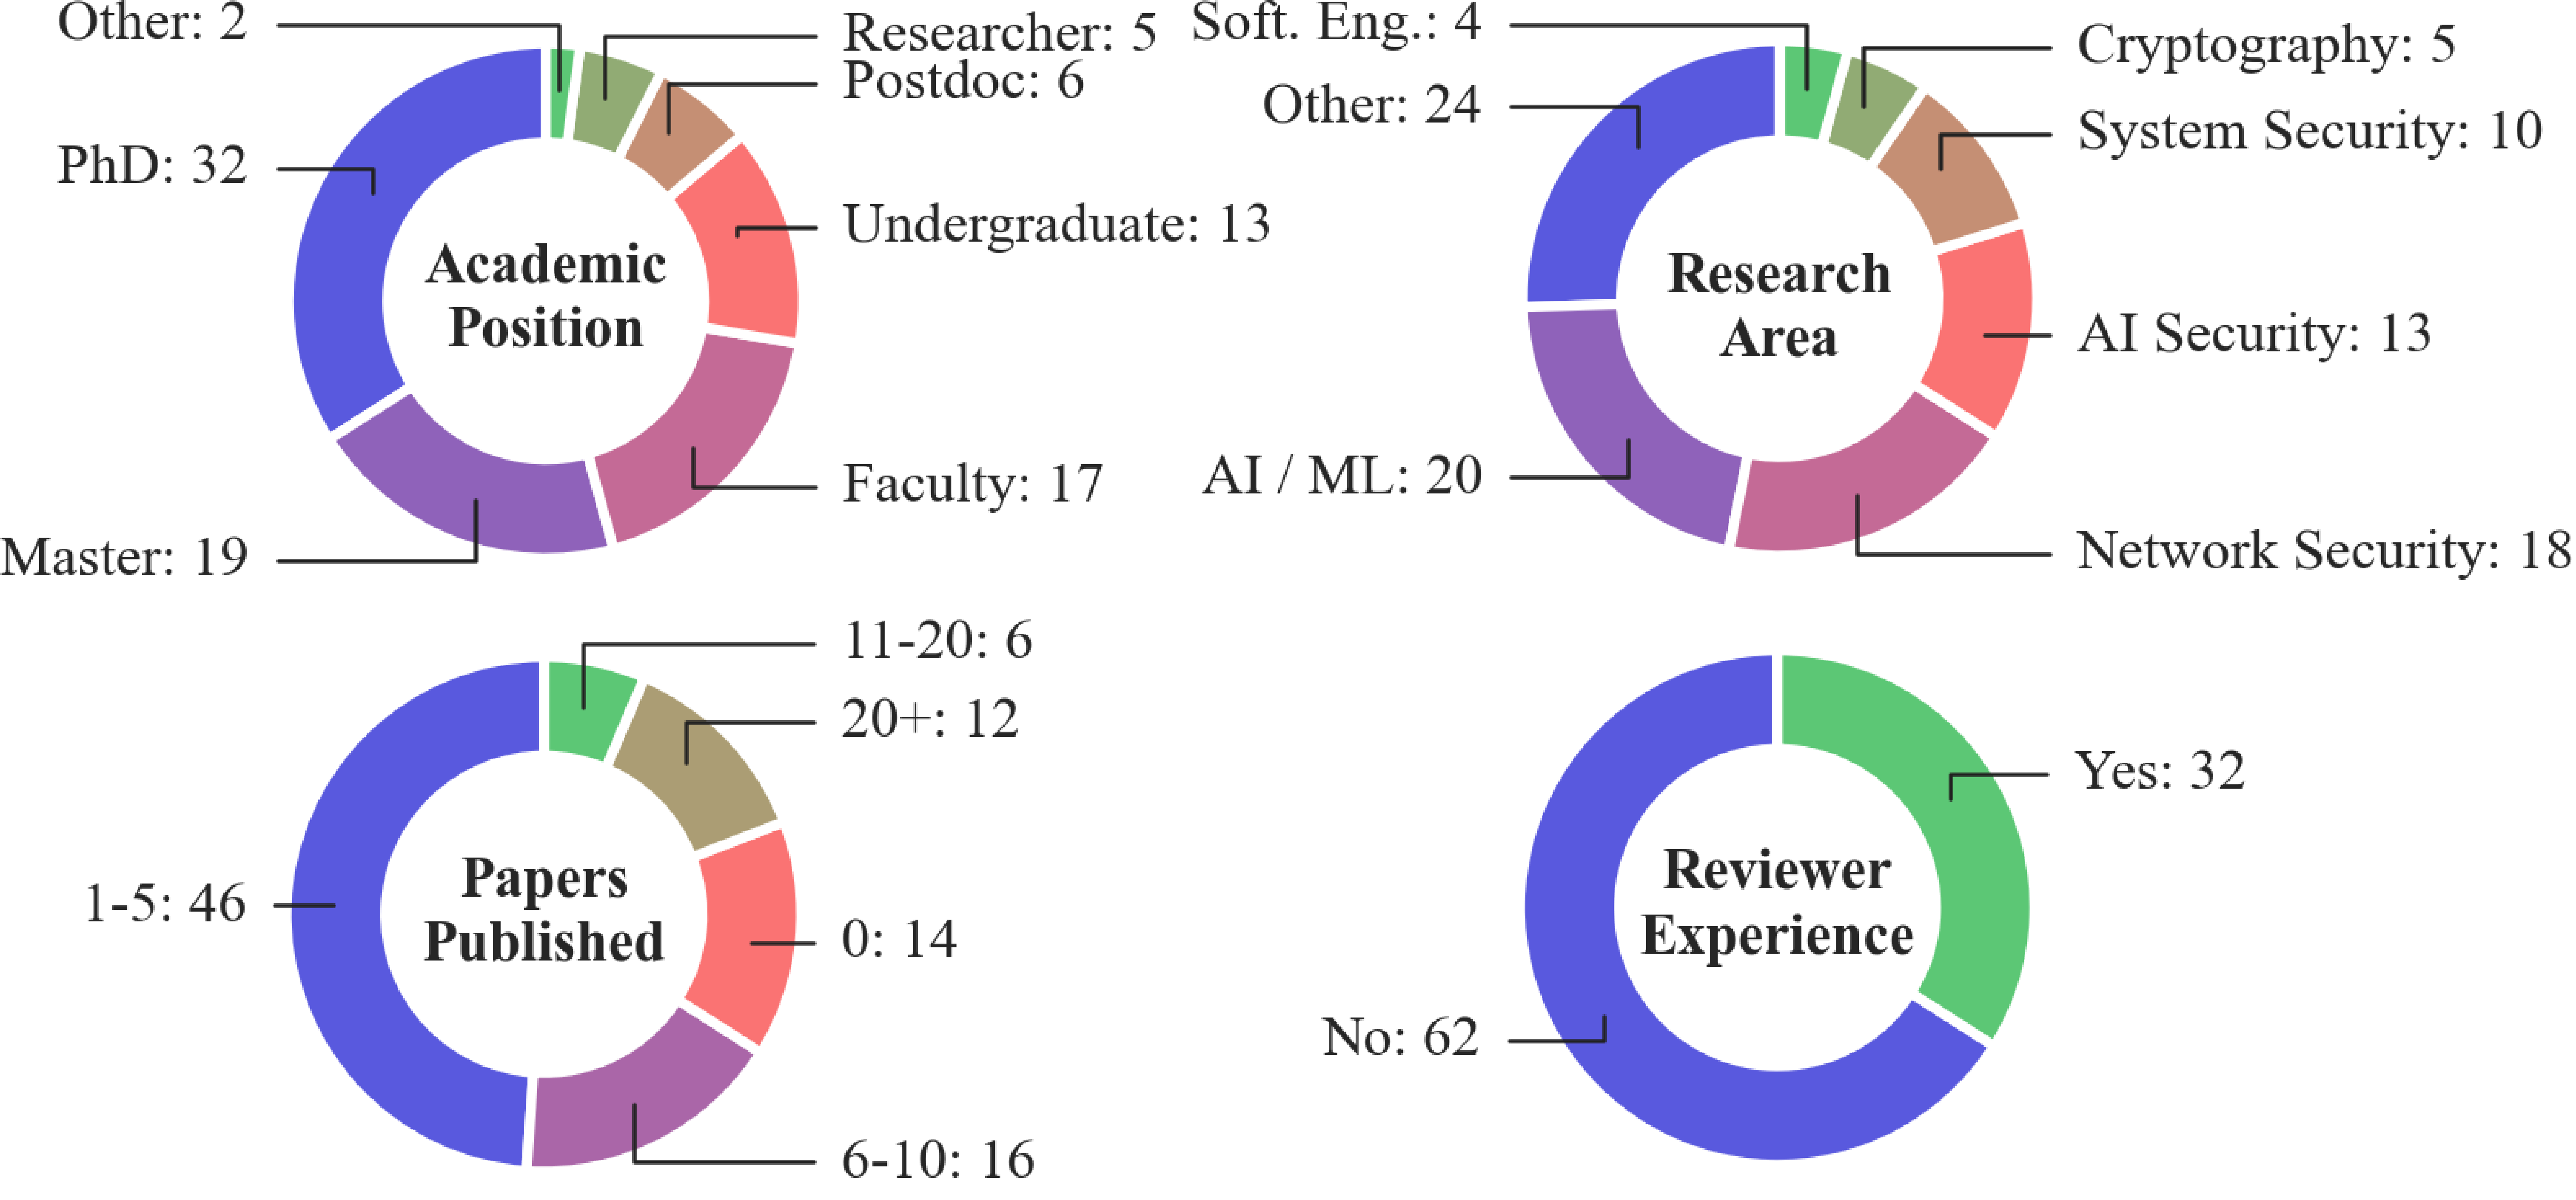
\includegraphics[width=0.5\textwidth]{figure/Sec7_Survey/profile_demographics.pdf}
    \caption{Demographic breakdown of 94 survey respondents by career stage, research area, and publication experience. Soft. Eng.: Software Engineering.}
    \label{fig:survey_profiles}
\end{figure}


\noindent
\textbf{Dataset Overview.}
We included paired reverse-worded BibTeX verification items to flag inconsistent responses.  
\cref{fig:survey_profiles} shows the demographic breakdown of our 94 respondents, spanning diverse career stages, research areas, and publication experience.
\cref{fig:survey_key_questions} summarizes the key findings across four dimensions; we discuss each below. 
The complete question wording, numbering and full response breakdown is illustrated in \cref{app:survey_details_full}.

\subsection{AI Adoption and Workflow Integration}

Our survey reveals widespread adoption of AI tools in academic research workflows.
Among respondents who answered the AI-use question (n=86), \textit{87.2\%} (75/86) report using AI-powered tools for research purposes.
This high adoption rate spans all career stages and research areas, indicating that AI assistance has become normalized in contemporary academic practice.

\noindent
\textbf{AI Tools Are Normalized in Academic Workflows.}
Among AI users, the majority employ these tools for text polishing:
46.7\% use AI for ``specific difficult paragraphs,''
29.3\% use it for ``almost every sentence,'' 22.7\% reserve it for ``final proofreading'' only,
and only 1.3\% (1/75) report not using AI for polishing.
This pervasive integration into the writing process creates multiple opportunities for AI-generated content (including citations) to enter manuscripts.

\noindent
\textbf{Most Researchers Rely on Google Scholar for References.}
When preparing references, most respondents rely on Google Scholar's ``Cite'' button (72.6\%), while 17.9\% export directly from publishers (e.g., IEEE/ACM), and 4.8\% copy BibTeX entries from other papers.
These behaviors increase exposure to propagation risks when upstream metadata contains errors.

%-------------------------------------------------------------------------------
\subsection{Verification Practices}

We next examine how researchers handle citations in practice, focusing on self-reported verification behaviors, risky citation habits, and perceptions of peer review efficacy.

\noindent
\textbf{Researchers Trust Citations by Default.}
Among authors, \textit{41.5\%} (39/94) copy-paste BibTeX without checking, and \textit{17.3\%} (13/75) cite AI-suggested papers without reading them. Among reviewers (n=30), \textit{76.7\%} do not thoroughly check references, and 80.0\% report never suspecting fake or hallucinated references in submissions.

This trust-by-default norm persists despite high exposure to hallucinated citations: \textit{41.3\%} (31/75) of AI users encounter them ``often'' or ``very often''. Respondents also view peer review as weak protection: 74.5\% combined rate citation error detection as ``not very effective'' or ``ineffective''. And when encountering suspicious references, 44.4\% choose no-action options (verify privately or ignore).

Figure~\ref{fig:survey_key_questions} summarizes these key questions spanning AI adoption, reporting behavior, peer review efficacy, and support for automated checks.

% Figure: Key survey questions (2x2)
\begin{figure}[t]
    \centering
    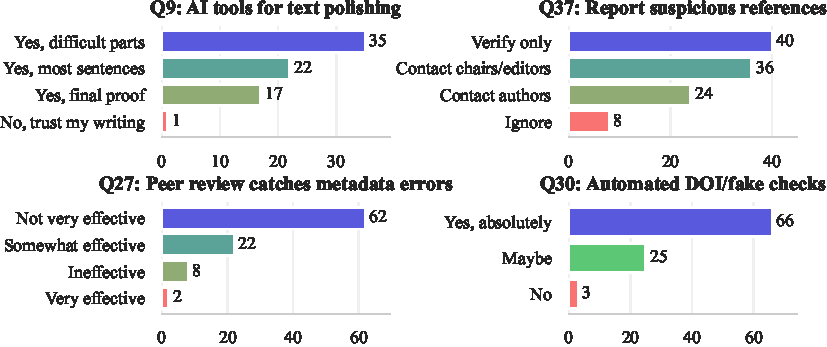
\includegraphics[width=\columnwidth]{figure/Sec7_Survey/key_questions_2x2.pdf}
    \caption{Summary of key survey findings across four dimensions: AI adoption, reporting behavior, peer review efficacy, and support for automated checks.}
     \label{fig:survey_key_questions}
\end{figure}


%-------------------------------------------------------------------------------
\subsection{Perception of Severity and Responsibility}

The research community demonstrates awareness of citation integrity issues.
\textit{76.6\%} of respondents (72/94) consider hallucinated citations a ``major problem'' or ``critical crisis,'' with 44.7\% rating it as a critical crisis and 31.9\% as a major problem.
This majority recognition of the problem's severity suggests that the persistence of hallucinated citations is not due to ignorance but rather to systemic factors in research workflows.

\noindent
\textbf{Accountability Falls on Authors Alone.}
When asked who bears primary responsibility for citation accuracy, \textit{91.5\%} (86/94) attribute responsibility to authors, while only 3.2\% assign it to reviewers, 2.1\% to publishers, and 2.1\% to AI tool developers.
This concentration of responsibility on authors leaves little perceived obligation for venues or tool developers to implement systemic safeguards.

\noindent
\textbf{Support for Automated Verification.}
Encouragingly, \textit{70.2\%} (66/94) strongly support deploying automated DOI/reference checking in submission systems, with an additional \textit{26.6\%} responding ``maybe.''
Only 3.2\% oppose such measures.
This strong support indicates community readiness for technological interventions to address citation integrity.

\begin{keyfindingsSidebar}{\faLightbulb\ Keyfinding 3: User Study}
\begin{itemize}
    \setlength{\itemsep}{-0pt}
    \setlength{\topsep}{0pt}
    \setlength{\partopsep}{0pt}
    \setlength{\parsep}{-0pt}
    \item \textit{87.2\%} of researchers use AI-powered tools in their workflows.
    \item Researchers trust citations by default: 41.5\% copy-paste BibTeX without checking, and 76.7\% of reviewers do not thoroughly inspect references.
    \item \textit{91.5\%} attribute citation accuracy responsibility to authors alone, potentially reducing pressure on other stakeholders.
    \item Peer review is viewed as ineffective at catching citation errors (74.5\%), whereas support for automated checks is strong (70.2\%).
\end{itemize}
\end{keyfindingsSidebar}

%-------------------------------------------------------------------------------
% \subsection{Reviewer Perspectives on Citation Errors}

% Our survey reveals how reviewers respond to citation errors, providing insight into peer review's role as a potential defense mechanism.

% \noindent
% \textbf{Single Citation Errors: Tolerated.}
% For a single wrong citation, the vast majority of reviewers (70.1\%) would merely ``mention it in minor comments,'' treating it as a fixable error rather than a serious concern.
% Only 4.1\% would reject the paper, and no reviewers would ignore it entirely.
% This lenient response to isolated errors means that papers with one or two hallucinated citations are unlikely to be caught during review.

% \noindent
% \textbf{Multiple Citation Errors: Treated as Ethical Violation.}
% The response changes dramatically when reviewers discover more than 5 wrong citations:
% \textit{46.4\% would reject immediately}, citing ethical concerns, and \textit{35.1\% would ask for an explanation before deciding.}
% Only 14.4\% would still treat it as a minor issue.
% Notably, \textit{no reviewers} would consider multiple errors an ``innocent mistake.''
% This threshold effect (where single errors are tolerated but clusters trigger rejection) aligns with our archival analysis finding that most papers with invalid citations contain only one error (Section~\ref{sec:archival_results}).
% Authors who limit their use of unverified AI-generated citations may stay below the detection threshold.

%-------------------------------------------------------------------------------
% \subsection{The Cognitive Offloading Hypothesis}

% Our survey findings support a \textit{cognitive offloading} explanation for why hallucinated citations persist despite researcher awareness.

% The combination of high AI adoption, perceived efficiency gains, and psychological tendency to trust automated outputs creates conditions where verification becomes perfunctory.
% Researchers may believe they are verifying citations while actually performing only superficial checks (e.g., confirming the title ``looks reasonable'') rather than rigorous validation (e.g., locating the actual paper).

